\documentclass[10pt,a4paper]{article}
\usepackage[utf8]{inputenc}
\usepackage[magyar]{babel}
\usepackage[T1]{fontenc}
\usepackage{amsmath}
\usepackage{amsfonts}
\usepackage{amssymb}
\usepackage{graphicx}
\begin{document}
\title{Méréstechnika laboratórium II 12.mérés jegyzőkönyv}
\author{Koncz István Márton\\\\A2754O}
\date{\today}
\maketitle
\newpage
\section{12. sz. laboratóriumi mérés}
	Mérés dátuma:\date{2017.09.11}
	\subsection{A mérés célja}
	A teljesítmény összetevőinek, jellemzőinek méréssel történő meghatározása.
A mérés hibáinak meghatározása, figyelembevétele.
	\subsection{Mérési feladatok}
		\subsubsection{A mérőpanelen található izzó teljesítmény-feszültség karakterisztikájának meghatározása! A teljesítménymérő
használatának megismerése.
A teljesítmény számítása ill. mérése hibáinak
meghatározása!}
Cél: A mérőpanelen található $24 V$, $60 W$-os izzó a
teljesítmény mérése teljesítménymérővel valamint
teljesítmény-feszültség karakterisztikájának
felvétele, váltakozó feszültségű táplálás esetén, $0$ –
$20 V$ tartományban $2 V$-os lépésenként.\\\\
A mérendő objektum:\begin{figure}[hbtp]
\centering
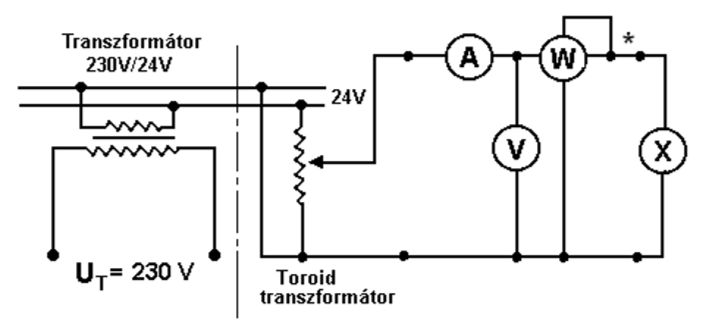
\includegraphics[scale=0.5]{Toroid.png}
\caption{}
\end{figure}\\\\
Mérési eredmények:


\begin{tabular}{|c|c|c|c|}
\hline 
Feszültség & Izzón átfolyó áram & Teljesítmény & Izzó számított ellenállása \\ 
\hline 
0V & &  &  \\ 
\hline 
2V &  &  & \\ 
\hline 
4V &  &  &  \\ 
\hline 
6V &  &  &  \\ 
\hline 
8V &  &  &  \\ 
\hline 
10V &  & &  \\ 
\hline 
12V & &  &  \\ 
\hline 
14V & & &  \\ 
\hline 
16V &  &  &  \\ 
\hline 
18V &  &  &  \\ 
\hline 
20V &  &  &  \\ 
\hline 
\end{tabular} \\\\


\newpage
A legnagyobb mért érték esetén a mérés bizonytalansága:$$\pm h_I=\pm $$ $$\pm h_U = \pm $$ $$h_P = h_I + h_U = $$
Az ábrák a $12.1$-es mellékletben vannak.\\\\
A mérési feladat értékelése:$$$$ $$$$ $$$$
			 \subsubsection{Teljesítmény mérés ohmos-induktív terhelés esetén}
A mérés során egy, az ohmos terheléssel (izzóval) sorosan kapcsolt tekercs hatását mérjük, úgy, hogy a vasmag kiszerelhetőségének segítségével változtatjuk a tekercs induktivitását.
A teljesítménymérővel a hatásos teljesítményt mérünk.\\\\
\begin{tabular}{|c|c|c|c|}
\hline 
\multicolumn{4}{|c|}{Vasmag nélkül} \\ 
\hline 
Tápfeszültség & Mért áram & Mért feszültség & Mért teljesítmény \\ 
\hline 
5V &  &  &  \\ 
\hline 
10V &  &  &  \\ 
\hline 
\end{tabular} \\\\
\\\\ 
\begin{tabular}{|c|c|c|c|}
\hline 
\multicolumn{4}{|c|}{Vasmaggal} \\ 
\hline 
Tápfeszültség & Mért áram & Mért feszültség & Mért teljesítmény \\ 
\hline 
5V &  &  &  \\ 
\hline 
10V &  &  &  \\ 
\hline 
\end{tabular}
\\\\
\\\\
\begin{tabular}{|c|c|c|c|}
\hline 
\multicolumn{4}{|c|}{Gumilappal a vasmag résében} \\ 
\hline 
Tápfeszültség & Mért áram & Mért feszültség & Mért teljesítmény \\ 
\hline 
5V &  &  &  \\ 
\hline 
10V &  &  &  \\ 
\hline 
\end{tabular}
\\\\
Számítások: 
\newpage
$$$$ $$$$ $$$$
Az ábrák a $12.2$-es mellékletben találhatóak meg.\\\\
A mérési feladat értékelése:$$$$ $$$$ $$$$
 \subsubsection{Pákatranszformátor kimeneti jelleggörbéjének felvétele}
 Számítsa ki a mérőhelyen található $20 VA$-s pákatranszformátor $24 V$-s
kimenetére vonatkozó névleges terhelő áram és terhelő ellenállás értékét. Mérje
meg a pákatranszformátor 24 V-s kimenetének üresjárási feszültségét! A
mellékelt tolóellenállás felhasználásával állítsa be a névleges terhelő áramot és
ismételje meg az előző mérést! A mért értékek alapján számítsa ki a
feszültségesés illetve a teljesítmény veszteség értékét. A mérés eredményét
ábrázolja $U_{ki}$, $I_{ki}$ koordinátarendszerben.
$$$$ 
Névleges áram:
$$$$ \\\\
Névleges feszültség:
$$$$
\\\\\begin{tabular}{|c|c|c|}
\hline 
Mérés & Tolóellenállás nélkül & Tolóellenállással \\ 
\hline 
Terhelő áram $I_t$ &  &  \\ 
\hline 
Terhelő áram $R_t$ &  &  \\ 
\hline 
Üresjárási feszültség $U_{kiü}$ &  &  \\ 
\hline 
\end{tabular} \\\\
Számítások:
\newpage
Az ábrák a $12.3$-as mellékletben vannak.
\\\\
A mérési feladat értékelése:$$$$ $$$$ $$$$
\tableofcontents
\end{document}